\documentclass[]{article}
\usepackage{lmodern}
\usepackage{amssymb,amsmath}
\usepackage{ifxetex,ifluatex}
\usepackage{fixltx2e} % provides \textsubscript
\ifnum 0\ifxetex 1\fi\ifluatex 1\fi=0 % if pdftex
  \usepackage[T1]{fontenc}
  \usepackage[utf8]{inputenc}
\else % if luatex or xelatex
  \ifxetex
    \usepackage{mathspec}
  \else
    \usepackage{fontspec}
  \fi
  \defaultfontfeatures{Ligatures=TeX,Scale=MatchLowercase}
\fi
% use upquote if available, for straight quotes in verbatim environments
\IfFileExists{upquote.sty}{\usepackage{upquote}}{}
% use microtype if available
\IfFileExists{microtype.sty}{%
\usepackage{microtype}
\UseMicrotypeSet[protrusion]{basicmath} % disable protrusion for tt fonts
}{}
\usepackage[margin=1in]{geometry}
\usepackage{hyperref}
\hypersetup{unicode=true,
            pdftitle={Problem Set 2},
            pdfborder={0 0 0},
            breaklinks=true}
\urlstyle{same}  % don't use monospace font for urls
\usepackage{color}
\usepackage{fancyvrb}
\newcommand{\VerbBar}{|}
\newcommand{\VERB}{\Verb[commandchars=\\\{\}]}
\DefineVerbatimEnvironment{Highlighting}{Verbatim}{commandchars=\\\{\}}
% Add ',fontsize=\small' for more characters per line
\usepackage{framed}
\definecolor{shadecolor}{RGB}{248,248,248}
\newenvironment{Shaded}{\begin{snugshade}}{\end{snugshade}}
\newcommand{\KeywordTok}[1]{\textcolor[rgb]{0.13,0.29,0.53}{\textbf{{#1}}}}
\newcommand{\DataTypeTok}[1]{\textcolor[rgb]{0.13,0.29,0.53}{{#1}}}
\newcommand{\DecValTok}[1]{\textcolor[rgb]{0.00,0.00,0.81}{{#1}}}
\newcommand{\BaseNTok}[1]{\textcolor[rgb]{0.00,0.00,0.81}{{#1}}}
\newcommand{\FloatTok}[1]{\textcolor[rgb]{0.00,0.00,0.81}{{#1}}}
\newcommand{\ConstantTok}[1]{\textcolor[rgb]{0.00,0.00,0.00}{{#1}}}
\newcommand{\CharTok}[1]{\textcolor[rgb]{0.31,0.60,0.02}{{#1}}}
\newcommand{\SpecialCharTok}[1]{\textcolor[rgb]{0.00,0.00,0.00}{{#1}}}
\newcommand{\StringTok}[1]{\textcolor[rgb]{0.31,0.60,0.02}{{#1}}}
\newcommand{\VerbatimStringTok}[1]{\textcolor[rgb]{0.31,0.60,0.02}{{#1}}}
\newcommand{\SpecialStringTok}[1]{\textcolor[rgb]{0.31,0.60,0.02}{{#1}}}
\newcommand{\ImportTok}[1]{{#1}}
\newcommand{\CommentTok}[1]{\textcolor[rgb]{0.56,0.35,0.01}{\textit{{#1}}}}
\newcommand{\DocumentationTok}[1]{\textcolor[rgb]{0.56,0.35,0.01}{\textbf{\textit{{#1}}}}}
\newcommand{\AnnotationTok}[1]{\textcolor[rgb]{0.56,0.35,0.01}{\textbf{\textit{{#1}}}}}
\newcommand{\CommentVarTok}[1]{\textcolor[rgb]{0.56,0.35,0.01}{\textbf{\textit{{#1}}}}}
\newcommand{\OtherTok}[1]{\textcolor[rgb]{0.56,0.35,0.01}{{#1}}}
\newcommand{\FunctionTok}[1]{\textcolor[rgb]{0.00,0.00,0.00}{{#1}}}
\newcommand{\VariableTok}[1]{\textcolor[rgb]{0.00,0.00,0.00}{{#1}}}
\newcommand{\ControlFlowTok}[1]{\textcolor[rgb]{0.13,0.29,0.53}{\textbf{{#1}}}}
\newcommand{\OperatorTok}[1]{\textcolor[rgb]{0.81,0.36,0.00}{\textbf{{#1}}}}
\newcommand{\BuiltInTok}[1]{{#1}}
\newcommand{\ExtensionTok}[1]{{#1}}
\newcommand{\PreprocessorTok}[1]{\textcolor[rgb]{0.56,0.35,0.01}{\textit{{#1}}}}
\newcommand{\AttributeTok}[1]{\textcolor[rgb]{0.77,0.63,0.00}{{#1}}}
\newcommand{\RegionMarkerTok}[1]{{#1}}
\newcommand{\InformationTok}[1]{\textcolor[rgb]{0.56,0.35,0.01}{\textbf{\textit{{#1}}}}}
\newcommand{\WarningTok}[1]{\textcolor[rgb]{0.56,0.35,0.01}{\textbf{\textit{{#1}}}}}
\newcommand{\AlertTok}[1]{\textcolor[rgb]{0.94,0.16,0.16}{{#1}}}
\newcommand{\ErrorTok}[1]{\textcolor[rgb]{0.64,0.00,0.00}{\textbf{{#1}}}}
\newcommand{\NormalTok}[1]{{#1}}
\usepackage{graphicx,grffile}
\makeatletter
\def\maxwidth{\ifdim\Gin@nat@width>\linewidth\linewidth\else\Gin@nat@width\fi}
\def\maxheight{\ifdim\Gin@nat@height>\textheight\textheight\else\Gin@nat@height\fi}
\makeatother
% Scale images if necessary, so that they will not overflow the page
% margins by default, and it is still possible to overwrite the defaults
% using explicit options in \includegraphics[width, height, ...]{}
\setkeys{Gin}{width=\maxwidth,height=\maxheight,keepaspectratio}
\IfFileExists{parskip.sty}{%
\usepackage{parskip}
}{% else
\setlength{\parindent}{0pt}
\setlength{\parskip}{6pt plus 2pt minus 1pt}
}
\setlength{\emergencystretch}{3em}  % prevent overfull lines
\providecommand{\tightlist}{%
  \setlength{\itemsep}{0pt}\setlength{\parskip}{0pt}}
\setcounter{secnumdepth}{0}
% Redefines (sub)paragraphs to behave more like sections
\ifx\paragraph\undefined\else
\let\oldparagraph\paragraph
\renewcommand{\paragraph}[1]{\oldparagraph{#1}\mbox{}}
\fi
\ifx\subparagraph\undefined\else
\let\oldsubparagraph\subparagraph
\renewcommand{\subparagraph}[1]{\oldsubparagraph{#1}\mbox{}}
\fi

%%% Use protect on footnotes to avoid problems with footnotes in titles
\let\rmarkdownfootnote\footnote%
\def\footnote{\protect\rmarkdownfootnote}

%%% Change title format to be more compact
\usepackage{titling}

% Create subtitle command for use in maketitle
\newcommand{\subtitle}[1]{
  \posttitle{
    \begin{center}\large#1\end{center}
    }
}

\setlength{\droptitle}{-2em}
  \title{Problem Set 2}
  \pretitle{\vspace{\droptitle}\centering\huge}
  \posttitle{\par}
  \author{}
  \preauthor{}\postauthor{}
  \date{}
  \predate{}\postdate{}


\begin{document}
\maketitle

\section{Population Genetics Problem Set
2}\label{population-genetics-problem-set-2}

\subsection{Sydney Wyatt}\label{sydney-wyatt}

\subsubsection{May 1, 2017}\label{may-1-2017}

\subsubsection{Question 1}\label{question-1}

\textbf{A) Use a program such as R or Excel to generate a scatter plot
that shows how expected allele frequency change from genetic drift
depends on initial allele frequency. The x-axis should be initial allele
frequency and range from 0 to 1. The y-axis should be expected change in
allele frequency after one generation. Perform calculations in steps of
0.1 for a population size of 2N=20.}

\begin{Shaded}
\begin{Highlighting}[]
\NormalTok{A.initialprob =}\StringTok{ }\KeywordTok{seq}\NormalTok{(}\FloatTok{0.1}\NormalTok{,}\DecValTok{1}\NormalTok{, }\DataTypeTok{by =} \FloatTok{0.1}\NormalTok{)}
\NormalTok{A.changingprob =}\StringTok{ }\KeywordTok{seq}\NormalTok{(}\DecValTok{0}\NormalTok{,}\DecValTok{1}\NormalTok{, }\DataTypeTok{by =} \FloatTok{0.1}\NormalTok{)}
\NormalTok{A.n =}\StringTok{ }\DecValTok{20}
\NormalTok{A.SecondGenExpChange =}\StringTok{ }\KeywordTok{c}\NormalTok{()}

\NormalTok{for(i in A.initialprob)\{}
  \NormalTok{expected.change =}\StringTok{ }\KeywordTok{c}\NormalTok{()}
  \NormalTok{for(p in }\KeywordTok{seq_along}\NormalTok{(A.changingprob))\{}
    \NormalTok{if (p==}\DecValTok{1}\NormalTok{)\{}
      \NormalTok{x =}\StringTok{ }\NormalTok{A.changingprob[p]*(}\KeywordTok{dbinom}\NormalTok{((}\DecValTok{20}\NormalTok{*A.changingprob[p]), }\DataTypeTok{size =} \NormalTok{A.n, }\DataTypeTok{prob =} \NormalTok{i) +}\StringTok{ }\KeywordTok{dbinom}\NormalTok{((}\DecValTok{20}\NormalTok{*A.changingprob[p]+}\DecValTok{1}\NormalTok{), }\DataTypeTok{size =} \NormalTok{A.n, }\DataTypeTok{prob =} \NormalTok{i))}
      \NormalTok{expected.change =}\StringTok{ }\KeywordTok{append}\NormalTok{(expected.change, x)\}}
    \NormalTok{else if (p==}\DecValTok{11}\NormalTok{)\{}
      \NormalTok{y =}\StringTok{ }\NormalTok{A.changingprob[p]*(}\KeywordTok{dbinom}\NormalTok{((}\DecValTok{20}\NormalTok{*A.changingprob[p]-}\DecValTok{1}\NormalTok{), }\DataTypeTok{size =} \NormalTok{A.n, }\DataTypeTok{prob =} \NormalTok{i) +}\StringTok{ }\KeywordTok{dbinom}\NormalTok{((}\DecValTok{20}\NormalTok{*A.changingprob[p]), }\DataTypeTok{size =} \NormalTok{A.n, }\DataTypeTok{prob =} \NormalTok{i))}
      \NormalTok{expected.change =}\StringTok{ }\KeywordTok{append}\NormalTok{(expected.change,y)\}}
    \NormalTok{else\{}
      \NormalTok{z =}\StringTok{ }\NormalTok{A.changingprob[p]*(}\KeywordTok{dbinom}\NormalTok{((}\DecValTok{20}\NormalTok{*A.changingprob[p]-}\DecValTok{1}\NormalTok{), }\DataTypeTok{size =} \NormalTok{A.n, }\DataTypeTok{prob =} \NormalTok{i) +}\StringTok{ }\KeywordTok{dbinom}\NormalTok{((}\DecValTok{20}\NormalTok{*A.changingprob[p]+}\DecValTok{1}\NormalTok{), }\DataTypeTok{size =} \NormalTok{A.n, }\DataTypeTok{prob =} \NormalTok{i))  }
      \NormalTok{expected.change =}\StringTok{ }\KeywordTok{append}\NormalTok{(expected.change,z)\}}
  \NormalTok{\}}
  \NormalTok{A.SecondGenExpChange =}\StringTok{ }\KeywordTok{append}\NormalTok{(A.SecondGenExpChange, }\KeywordTok{sum}\NormalTok{(expected.change))}
\NormalTok{\}}

\KeywordTok{library}\NormalTok{(CatterPlots)}
\end{Highlighting}
\end{Shaded}

\begin{verbatim}
## Loading required package: png
\end{verbatim}

\begin{verbatim}
## Warning: package 'png' was built under R version 3.2.5
\end{verbatim}

\begin{verbatim}
## 
## Welcome to CatterPlot.
\end{verbatim}

\begin{Shaded}
\begin{Highlighting}[]
\KeywordTok{catplot}\NormalTok{(A.initialprob, A.SecondGenExpChange, }\DataTypeTok{size =} \FloatTok{0.1}\NormalTok{, }\DataTypeTok{cat =} \DecValTok{11}\NormalTok{, }\DataTypeTok{xlab =} \StringTok{"Initial Allele Frequency"}\NormalTok{, }\DataTypeTok{ylab =} \StringTok{"New Allele Frequency"}\NormalTok{, }\DataTypeTok{main =} \StringTok{"Expected Change in Allele Frequency After One Generation"}\NormalTok{)}
\end{Highlighting}
\end{Shaded}

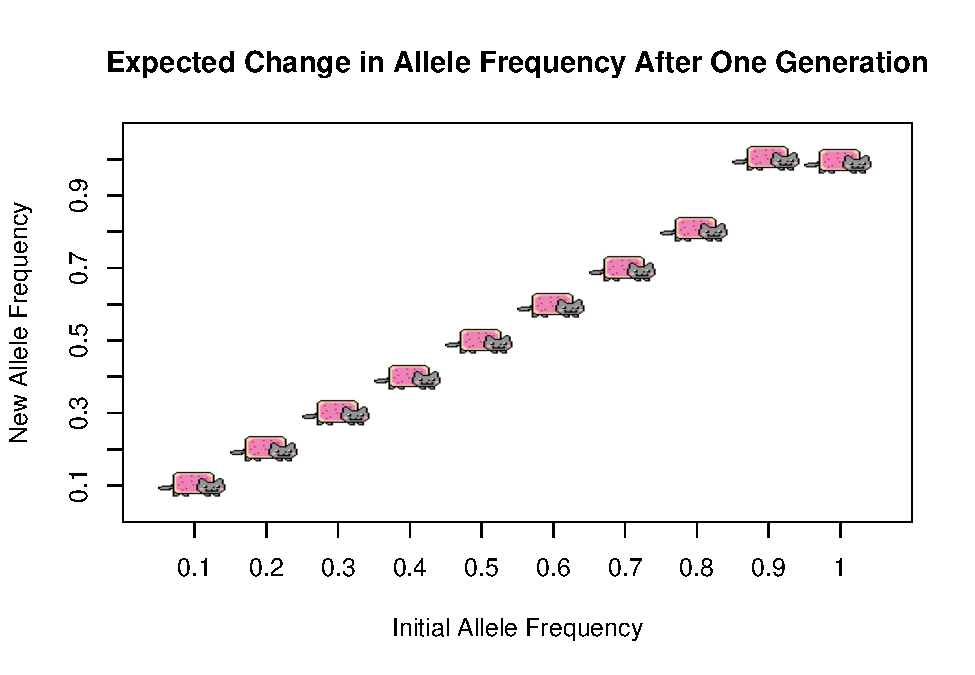
\includegraphics{Problem_Set_2_files/figure-latex/unnamed-chunk-1-1.pdf}

\begin{verbatim}
## $xs
##  [1] 0.1 0.2 0.3 0.4 0.5 0.6 0.7 0.8 0.9 1.0
## 
## $ys
##  [1] 0.1014412 0.2000122 0.3000000 0.4000000 0.5000010 0.6000366 0.7007979
##  [8] 0.8114805 1.0086063 1.0000000
## 
## $args
## $args$xlab
## [1] "Initial Allele Frequency"
## 
## $args$ylab
## [1] "New Allele Frequency"
## 
## $args$main
## [1] "Expected Change in Allele Frequency After One Generation"
## 
## 
## $canvas
## [1] 0.0 1.1 0.0 1.1
\end{verbatim}

\begin{Shaded}
\begin{Highlighting}[]
\CommentTok{#Simple for and if else loops:}
\CommentTok{#Not.Div = c()}
\CommentTok{#Div = c()}
\CommentTok{#for(i in 1:10)\{}
\CommentTok{#  if (i %% 4)\{}
\CommentTok{#    Not.Div = append(Not.Div,i)\}}
\CommentTok{#  else \{}
\CommentTok{#    Div = append(Div, i)\}}
\CommentTok{#\}}
\end{Highlighting}
\end{Shaded}

\textbf{B) Use the same program to generate a scatter plot that shows
how expected allele frequency change from genetic drift depends on
population size. The x-axis should be population size and range from
2N=10 to 2N=100. The y-axis should be expected change in allele
frequency after one generation. Perform calculations in steps of 10 with
an allele frequency of 0.5.}

\subsubsection{Question 2}\label{question-2}

\textbf{A) Use the same program to generate a scatter plot that shows
the properties of selection in large populations. The x-axis should be
frequency of the advantageous allele and range from 0 to 1. The y-axis
should be the change in frequency of the advantageous allele after one
generation of selection. Perform calculations in steps of 0.01 for each
of the following six (1a, 1b, 1c, 2a, 2b, 2c) scenarios: (1) the
homozygous deleterious genotype has a selection coefficient of 0.1 and
the advantageous allele is (a) recessive, (b) dominant or (c) additive;
(2) the homozygous deleterious genotype has a selection coefficient of
0.25 and the advantageous allele is (a) recessive, (b) dominant or (c)
additive.}

\textbf{B) Four of the six plots from above are highly asymmetric.
Explain the biological reason behind these asymmetric patterns.}


\end{document}
